\documentclass[11pt,fleqn]{book} % Default font size and left-justified equations

\usepackage[top=3cm,bottom=3cm,left=3.2cm,right=3.2cm,headsep=10pt,letterpaper]{geometry} % Page margins
\usepackage{float}
\usepackage{xcolor} % Required for specifying colors by name
\definecolor{ocre}{RGB}{52,177,201} % Define the orange color used for highlighting throughout the book

% Font Settings
\usepackage{avant} % Use the Avantgarde font for headings
%\usepackage{times} % Use the Times font for headings
\usepackage{mathptmx} % Use the Adobe Times Roman as the default text font together with math symbols from the Sym­bol, Chancery and Com­puter Modern fonts

\usepackage{microtype} % Slightly tweak font spacing for aesthetics
\usepackage[utf8]{inputenc} % Required for including letters with accents
\usepackage[T1]{fontenc} % Use 8-bit encoding that has 256 glyphs

% Bibliography
\usepackage[style=alphabetic,sorting=nyt,sortcites=true,autopunct=true,babel=hyphen,hyperref=true,abbreviate=false,backref=true,backend=biber]{biblatex}
\addbibresource{bibliography.bib} % BibTeX bibliography file
\defbibheading{bibempty}{}

%----------------------------------------------------------------------------------------
%	VARIOUS REQUIRED PACKAGES
%----------------------------------------------------------------------------------------

\usepackage{titlesec} % Allows customization of titles

\usepackage{graphicx} % Required for including pictures
\graphicspath{{Pictures/}} % Specifies the directory where pictures are stored

\usepackage{lipsum} % Inserts dummy text

\usepackage{tikz} % Required for drawing custom shapes

%\usepackage[english]{babel} % English language/hyphenation
\usepackage[german]{babel}

\usepackage{enumitem} % Customize lists
\setlist{nolistsep} % Reduce spacing between bullet points and numbered lists

\usepackage{booktabs} % Required for nicer horizontal rules in tables

\usepackage{eso-pic} % Required for specifying an image background in the title page

%----------------------------------------------------------------------------------------
%	MAIN TABLE OF CONTENTS
%----------------------------------------------------------------------------------------

\usepackage{titletoc} % Required for manipulating the table of contents

\contentsmargin{0cm} % Removes the default margin
% Chapter text styling
\titlecontents{chapter}[1.25cm] % Indentation
{\addvspace{15pt}\large\sffamily\bfseries} % Spacing and font options for chapters
{\color{ocre!60}\contentslabel[\Large\thecontentslabel]{1.25cm}\color{ocre}} % Chapter number
{}  
{\color{ocre!60}\normalsize\sffamily\bfseries\;\titlerule*[.5pc]{.}\;\thecontentspage} % Page number
% Section text styling
\titlecontents{section}[1.25cm] % Indentation
{\addvspace{5pt}\sffamily\bfseries} % Spacing and font options for sections
{\contentslabel[\thecontentslabel]{1.25cm}} % Section number
{}
{\sffamily\hfill\color{black}\thecontentspage} % Page number
[]
% Subsection text styling
\titlecontents{subsection}[1.25cm] % Indentation
{\addvspace{1pt}\sffamily\small} % Spacing and font options for subsections
{\contentslabel[\thecontentslabel]{1.25cm}} % Subsection number
{}
{\sffamily\;\titlerule*[.5pc]{.}\;\thecontentspage} % Page number
[] 

%----------------------------------------------------------------------------------------
%	MINI TABLE OF CONTENTS IN CHAPTER HEADS
%----------------------------------------------------------------------------------------

% Section text styling
\titlecontents{lsection}[0em] % Indendating
{\footnotesize\sffamily} % Font settings
{}
{}
{}

% Subsection text styling
\titlecontents{lsubsection}[.5em] % Indentation
{\normalfont\footnotesize\sffamily} % Font settings
{}
{}
{}
 
%----------------------------------------------------------------------------------------
%	PAGE HEADERS
%----------------------------------------------------------------------------------------

\usepackage{fancyhdr} % Required for header and footer configuration

\pagestyle{fancy}
\renewcommand{\chaptermark}[1]{\markboth{\sffamily\normalsize\bfseries\chaptername\ \thechapter.\ #1}{}} % Chapter text font settings
\renewcommand{\sectionmark}[1]{\markright{\sffamily\normalsize\thesection\hspace{5pt}#1}{}} % Section text font settings
\fancyhf{} \fancyhead[LE,RO]{\sffamily\normalsize\thepage} % Font setting for the page number in the header
\fancyhead[LO]{\rightmark} % Print the nearest section name on the left side of odd pages
\fancyhead[RE]{\leftmark} % Print the current chapter name on the right side of even pages
\renewcommand{\headrulewidth}{0.5pt} % Width of the rule under the header
\addtolength{\headheight}{2.5pt} % Increase the spacing around the header slightly
\renewcommand{\footrulewidth}{0pt} % Removes the rule in the footer
\fancypagestyle{plain}{\fancyhead{}\renewcommand{\headrulewidth}{0pt}} % Style for when a plain pagestyle is specified

% Removes the header from odd empty pages at the end of chapters
\makeatletter
\renewcommand{\cleardoublepage}{
\clearpage\ifodd\c@page\else
\hbox{}
\vspace*{\fill}
\thispagestyle{empty}
\newpage
\fi}

%----------------------------------------------------------------------------------------
%	THEOREM STYLES
%----------------------------------------------------------------------------------------

\usepackage{amsmath,amsfonts,amssymb,amsthm} % For math equations, theorems, symbols, etc

\newcommand{\intoo}[2]{\mathopen{]}#1\,;#2\mathclose{[}}
\newcommand{\ud}{\mathop{\mathrm{{}d}}\mathopen{}}
\newcommand{\intff}[2]{\mathopen{[}#1\,;#2\mathclose{]}}
\newtheorem{notation}{Notation}[chapter]

%%%%%%%%%%%%%%%%%%%%%%%%%%%%%%%%%%%%%%%%%%%%%%%%%%%%%%%%%%%%%%%%%%%%%%%%%%%
%%%%%%%%%%%%%%%%%%%% dedicated to boxed/framed environements %%%%%%%%%%%%%%
%%%%%%%%%%%%%%%%%%%%%%%%%%%%%%%%%%%%%%%%%%%%%%%%%%%%%%%%%%%%%%%%%%%%%%%%%%%
\newtheoremstyle{ocrenumbox}% % Theorem style name
{0pt}% Space above
{0pt}% Space below
{\normalfont}% % Body font
{}% Indent amount
{\small\bf\sffamily\color{ocre}}% % Theorem head font
{\;}% Punctuation after theorem head
{0.25em}% Space after theorem head
{\small\sffamily\color{ocre}\thmname{#1}\nobreakspace\thmnumber{\@ifnotempty{#1}{}\@upn{#2}}% Theorem text (e.g. Theorem 2.1)
\thmnote{\nobreakspace\the\thm@notefont\sffamily\bfseries\color{black}---\nobreakspace#3.}} % Optional theorem note
\renewcommand{\qedsymbol}{$\blacksquare$}% Optional qed square

\newtheoremstyle{blacknumex}% Theorem style name
{5pt}% Space above
{5pt}% Space below
{\normalfont}% Body font
{} % Indent amount
{\small\bf\sffamily}% Theorem head font
{\;}% Punctuation after theorem head
{0.25em}% Space after theorem head
{\small\sffamily{\tiny\ensuremath{\blacksquare}}\nobreakspace\thmname{#1}\nobreakspace\thmnumber{\@ifnotempty{#1}{}\@upn{#2}}% Theorem text (e.g. Theorem 2.1)
\thmnote{\nobreakspace\the\thm@notefont\sffamily\bfseries---\nobreakspace#3.}}% Optional theorem note

\newtheoremstyle{blacknumbox} % Theorem style name
{0pt}% Space above
{0pt}% Space below
{\normalfont}% Body font
{}% Indent amount
{\small\bf\sffamily}% Theorem head font
{\;}% Punctuation after theorem head
{0.25em}% Space after theorem head
{\small\sffamily\thmname{#1}\nobreakspace\thmnumber{\@ifnotempty{#1}{}\@upn{#2}}% Theorem text (e.g. Theorem 2.1)
\thmnote{\nobreakspace\the\thm@notefont\sffamily\bfseries---\nobreakspace#3.}}% Optional theorem note

%%%%%%%%%%%%%%%%%%%%%%%%%%%%%%%%%%%%%%%%%%%%%%%%%%%%%%%%%%%%%%%%%%%%%%%%%%%
%%%%%%%%%%%%% dedicated to non-boxed/non-framed environements %%%%%%%%%%%%%
%%%%%%%%%%%%%%%%%%%%%%%%%%%%%%%%%%%%%%%%%%%%%%%%%%%%%%%%%%%%%%%%%%%%%%%%%%%
\newtheoremstyle{ocrenum}% % Theorem style name
{5pt}% Space above
{5pt}% Space below
{\normalfont}% % Body font
{}% Indent amount
{\small\bf\sffamily\color{ocre}}% % Theorem head font
{\;}% Punctuation after theorem head
{0.25em}% Space after theorem head
{\small\sffamily\color{ocre}\thmname{#1}\nobreakspace\thmnumber{\@ifnotempty{#1}{}\@upn{#2}}% Theorem text (e.g. Theorem 2.1)
\thmnote{\nobreakspace\the\thm@notefont\sffamily\bfseries\color{black}---\nobreakspace#3.}} % Optional theorem note
\renewcommand{\qedsymbol}{$\blacksquare$}% Optional qed square
\makeatother

% Defines the theorem text style for each type of theorem to one of the three styles above
\newcounter{dummy} 
\numberwithin{dummy}{section}
\theoremstyle{ocrenumbox}
\newtheorem{theoremeT}[dummy]{Theorem}
\newtheorem{problem}{Problem}[chapter]
\newtheorem{exerciseT}{Exercise}[chapter]
\theoremstyle{blacknumex}
\newtheorem{exampleT}{Example}[chapter]
\theoremstyle{blacknumbox}
\newtheorem{vocabulary}{Vocabulary}[chapter]
\newtheorem{definitionT}{Definition}[section]
\newtheorem{corollaryT}[dummy]{Corollary}
\theoremstyle{ocrenum}
\newtheorem{proposition}[dummy]{Proposition}

%----------------------------------------------------------------------------------------
%	DEFINITION OF COLORED BOXES
%----------------------------------------------------------------------------------------

\RequirePackage[framemethod=default]{mdframed} % Required for creating the theorem, definition, exercise and corollary boxes

% Theorem box
\newmdenv[skipabove=7pt,
skipbelow=7pt,
backgroundcolor=black!5,
linecolor=ocre,
innerleftmargin=5pt,
innerrightmargin=5pt,
innertopmargin=5pt,
leftmargin=0cm,
rightmargin=0cm,
innerbottommargin=5pt]{tBox}

% Exercise box	  
\newmdenv[skipabove=7pt,
skipbelow=7pt,
rightline=false,
leftline=true,
topline=false,
bottomline=false,
backgroundcolor=ocre!10,
linecolor=ocre,
innerleftmargin=5pt,
innerrightmargin=5pt,
innertopmargin=5pt,
innerbottommargin=5pt,
leftmargin=0cm,
rightmargin=0cm,
linewidth=4pt]{eBox}	

% Definition box
\newmdenv[skipabove=7pt,
skipbelow=7pt,
rightline=false,
leftline=true,
topline=false,
bottomline=false,
linecolor=ocre,
innerleftmargin=5pt,
innerrightmargin=5pt,
innertopmargin=0pt,
leftmargin=0cm,
rightmargin=0cm,
linewidth=4pt,
innerbottommargin=0pt]{dBox}	

% Corollary box
\newmdenv[skipabove=7pt,
skipbelow=7pt,
rightline=false,
leftline=true,
topline=false,
bottomline=false,
linecolor=gray,
backgroundcolor=black!5,
innerleftmargin=5pt,
innerrightmargin=5pt,
innertopmargin=5pt,
leftmargin=0cm,
rightmargin=0cm,
linewidth=4pt,
innerbottommargin=5pt]{cBox}

% Creates an environment for each type of theorem and assigns it a theorem text style from the "Theorem Styles" section above and a colored box from above
\newenvironment{theorem}{\begin{tBox}\begin{theoremeT}}{\end{theoremeT}\end{tBox}}
\newenvironment{exercise}{\begin{eBox}\begin{exerciseT}}{\hfill{\color{ocre}\tiny\ensuremath{\blacksquare}}\end{exerciseT}\end{eBox}}				  
\newenvironment{definition}{\begin{dBox}\begin{definitionT}}{\end{definitionT}\end{dBox}}	
\newenvironment{example}{\begin{exampleT}}{\hfill{\tiny\ensuremath{\blacksquare}}\end{exampleT}}		
\newenvironment{corollary}{\begin{cBox}\begin{corollaryT}}{\end{corollaryT}\end{cBox}}	

%----------------------------------------------------------------------------------------
%	REMARK ENVIRONMENT
%----------------------------------------------------------------------------------------

\newenvironment{remark}{\par\vspace{10pt}\small % Vertical white space above the remark and smaller font size
\begin{list}{}{
\leftmargin=35pt % Indentation on the left
\rightmargin=25pt}\item\ignorespaces % Indentation on the right
\makebox[-2.5pt]{\begin{tikzpicture}[overlay]
\node[draw=ocre!60,line width=1pt,circle,fill=ocre!25,font=\sffamily\bfseries,inner sep=2pt,outer sep=0pt] at (-15pt,0pt){\textcolor{ocre}{R}};\end{tikzpicture}} % Orange R in a circle
\advance\baselineskip -1pt}{\end{list}\vskip5pt} % Tighter line spacing and white space after remark

%----------------------------------------------------------------------------------------
%	SECTION NUMBERING IN THE MARGIN
%----------------------------------------------------------------------------------------

\makeatletter
\renewcommand{\@seccntformat}[1]{\llap{\textcolor{ocre}{\csname the#1\endcsname}\hspace{1em}}}                    
\renewcommand{\section}{\@startsection{section}{1}{\z@}
{-4ex \@plus -1ex \@minus -.4ex}
{1ex \@plus.2ex }
{\normalfont\large\sffamily\bfseries}}
\renewcommand{\subsection}{\@startsection {subsection}{2}{\z@}
{-3ex \@plus -0.1ex \@minus -.4ex}
{0.5ex \@plus.2ex }
{\normalfont\sffamily\bfseries}}
\renewcommand{\subsubsection}{\@startsection {subsubsection}{3}{\z@}
{-2ex \@plus -0.1ex \@minus -.2ex}
{.2ex \@plus.2ex }
{\normalfont\small\sffamily\bfseries}}                        
\renewcommand\paragraph{\@startsection{paragraph}{4}{\z@}
{-2ex \@plus-.2ex \@minus .2ex}
{.1ex}
{\normalfont\small\sffamily\bfseries}}

%----------------------------------------------------------------------------------------
%	HYPERLINKS IN THE DOCUMENTS
%----------------------------------------------------------------------------------------

% For an unclear reason, the package should be loaded now and not later
\usepackage{hyperref}
\hypersetup{hidelinks,backref=true,pagebackref=true,hyperindex=true,colorlinks=false,breaklinks=true,urlcolor= ocre,bookmarks=true,bookmarksopen=false,pdftitle={Title},pdfauthor={Author}}

%----------------------------------------------------------------------------------------
%	CHAPTER HEADINGS
%----------------------------------------------------------------------------------------

% The set-up below should be (sadly) manually adapted to the overall margin page septup controlled by the geometry package loaded in the main.tex document. It is possible to implement below the dimensions used in the goemetry package (top,bottom,left,right)... TO BE DONE

\newcommand{\thechapterimage}{}
\newcommand{\chapterimage}[1]{\renewcommand{\thechapterimage}{#1}}

% Numbered chapters with mini tableofcontents
\def\thechapter{\arabic{chapter}}
\def\@makechapterhead#1{
\thispagestyle{empty}
{\centering \normalfont\sffamily
\ifnum \c@secnumdepth >\m@ne
\if@mainmatter
\startcontents
\begin{tikzpicture}[remember picture,overlay]
\node at (current page.north west)
{\begin{tikzpicture}[remember picture,overlay]
\node[anchor=north west,inner sep=0pt] at (0,0) {\includegraphics[width=\paperwidth]{\thechapterimage}};
%%%%%%%%%%%%%%%%%%%%%%%%%%%%%%%%%%%%%%%%%%%%%%%%%%%%%%%%%%%%%%%%%%%%%%%%%%%%%%%%%%%%%
% Commenting the 3 lines below removes the small contents box in the chapter heading
%\fill[color=ocre!10!white,opacity=.6] (1cm,0) rectangle (8cm,-7cm);
%\node[anchor=north west] at (1.1cm,.35cm) {\parbox[t][8cm][t]{6.5cm}{\huge\bfseries\flushleft \printcontents{l}{1}{\setcounter{tocdepth}{2}}}};
\draw[anchor=west] (5cm,-9cm) node [rounded corners=20pt,fill=ocre!10!white,text opacity=1,draw=ocre,draw opacity=1,line width=1.5pt,fill opacity=.6,inner sep=12pt]{\huge\sffamily\bfseries\textcolor{black}{\thechapter. #1\strut\makebox[22cm]{}}};
%%%%%%%%%%%%%%%%%%%%%%%%%%%%%%%%%%%%%%%%%%%%%%%%%%%%%%%%%%%%%%%%%%%%%%%%%%%%%%%%%%%%%
\end{tikzpicture}};
\end{tikzpicture}}
\par\vspace*{230\p@}
\fi
\fi}

% Unnumbered chapters without mini tableofcontents (could be added though) 
\def\@makeschapterhead#1{
\thispagestyle{empty}
{\centering \normalfont\sffamily
\ifnum \c@secnumdepth >\m@ne
\if@mainmatter
\begin{tikzpicture}[remember picture,overlay]
\node at (current page.north west)
{\begin{tikzpicture}[remember picture,overlay]
\node[anchor=north west,inner sep=0pt] at (0,0) {\includegraphics[width=\paperwidth]{\thechapterimage}};
\draw[anchor=west] (5cm,-9cm) node [rounded corners=20pt,fill=ocre!10!white,fill opacity=.6,inner sep=12pt,text opacity=1,draw=ocre,draw opacity=1,line width=1.5pt]{\huge\sffamily\bfseries\textcolor{black}{#1\strut\makebox[22cm]{}}};
\end{tikzpicture}};
\end{tikzpicture}}
\par\vspace*{230\p@}
\fi
\fi
}
\makeatother % Insert the commands.tex file which contains the majority of the structure behind the template

\begin{document}


%	TITELSEITE

\begingroup
\thispagestyle{empty}
\AddToShipoutPicture*{\put(0,0){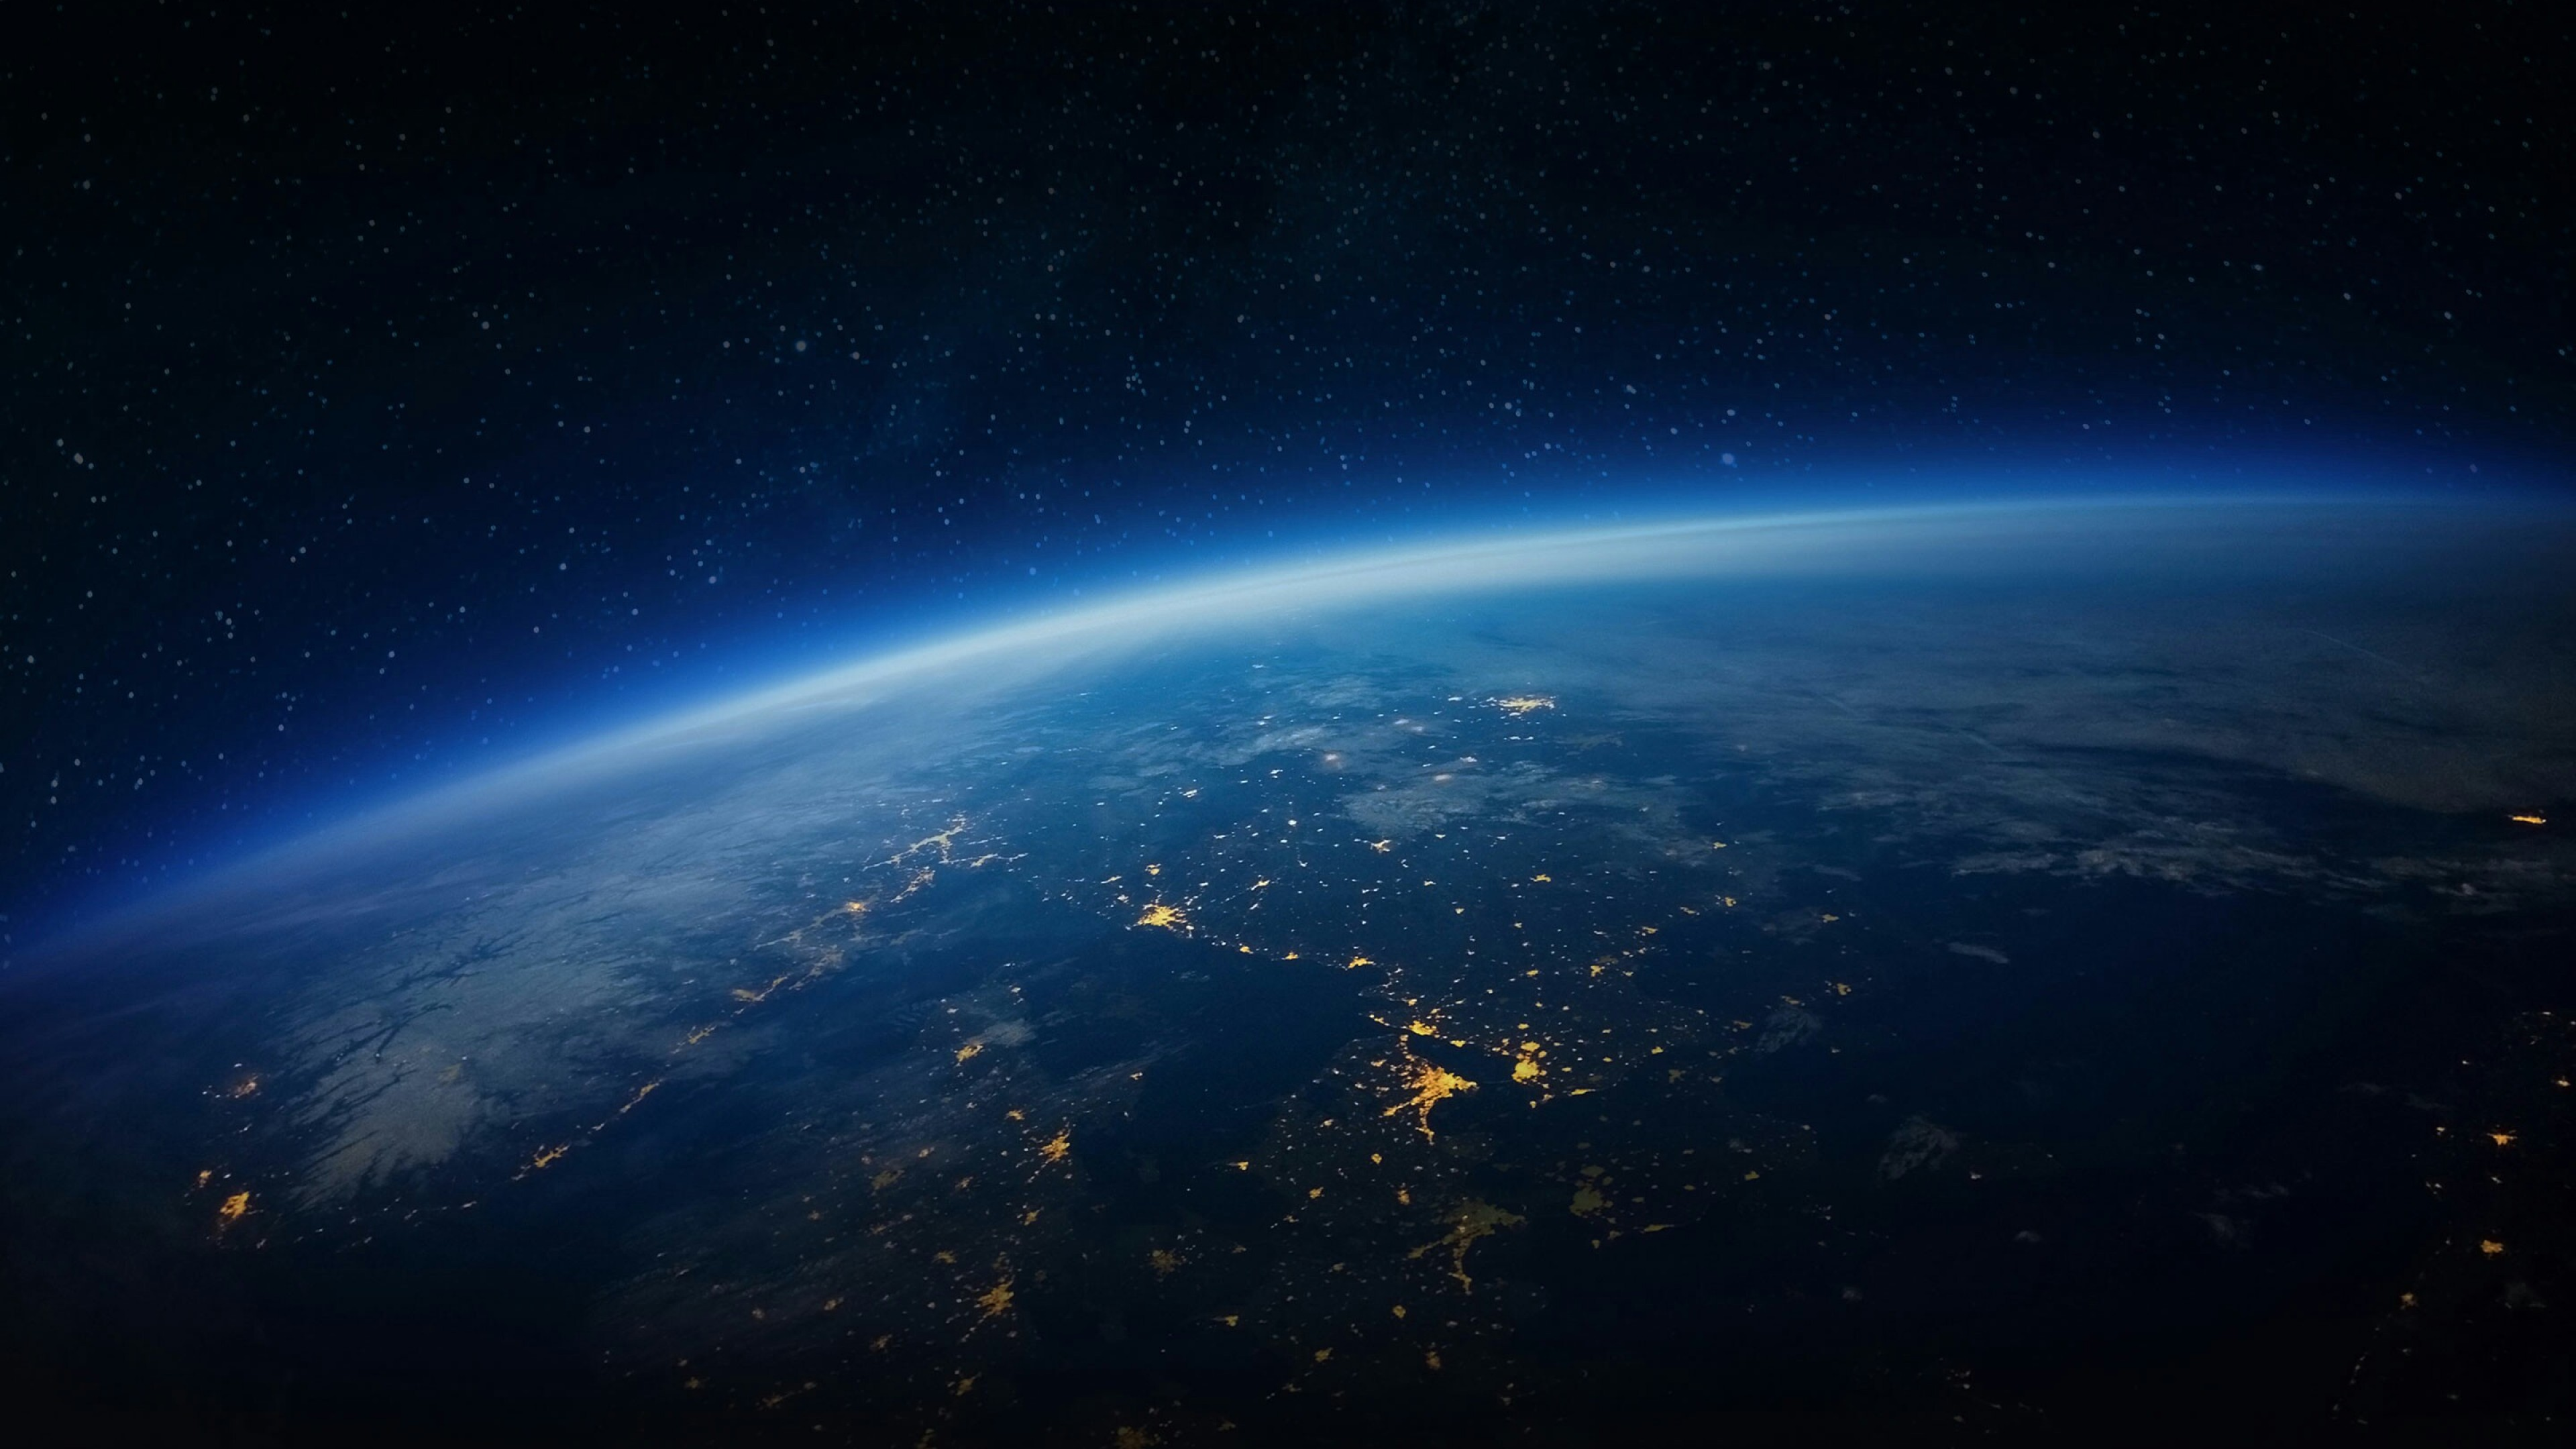
\includegraphics[scale=0.37]{head1.jpg}}} % Image background
\centering
\vspace*{5cm}
\par\normalfont\fontsize{35}{35}\sffamily\selectfont
\textbf{{\color{white} Neuronale Netzwerke und Clusteringverfahren für Geodaten}}\\
{\LARGE {\color{white}Lehrstuhl für Geoinformatik}}\par
\vspace*{1cm}
{\Huge {\color{white} Robin Bially}}\par % Author name
\endgroup

\newpage
~\vfill
\thispagestyle{empty}

%Hier kann ich Github und Downloads hin schreiben
\noindent \textsc{https://github.com/RobinBia/Projektarbeit-Geoinformatik.git}\\ % URL

\noindent Projektarbeit unter der Betreuung von PD Dr. Dr.-Ing. Wilfried Linder von 11.2017 - 09.2018 als Vorbereitung der sich anschließenden Masterarbeit.\\ 

\noindent \textit{Fertigstellung, August 2018} 

%	Inhaltsverzeichnis
\chapterimage{head8.jpg} % Table of contents heading image
\tableofcontents % Print the table of contents itself

%\cleardoublepage

\pagestyle{fancy} % Print headers again

\chapter{Motivation}
\chapter{Geodaten und Geoinformation}
\section{Definition und Gestalt von Geodaten}
Geodaten sind digitale Informationen, welche Sachdaten mit Geometriedaten\footnote{https://www.hdm-stuttgart.de/~riekert/lehre gis.pdf} (und Chronometriedaten) vereinen , z.B. \{Luftdruck 1 bar, Ort Düsseldorf, Datum 26.11.2017\}. 
Die räumliche Information kann in unterschiedlichen Formen vorliegen, z.B. symbolisch als Ortsname oder Postleitzahl, aber auch als mathematisch atomare Referenz auf Positionen der Erde mittels Koordinaten. Diese können in unterschiedlichster Dimensionalität vorliegen\footnote{http://www.mathematik.uni-ulm.de/sai/ws04/biosem/GIS.pdf}
\begin{itemize}
\item Ein Objekt ohne bestimmte Länge (0D)
\item Ein Linienstück (1D)
\item
Gauß-Krüger oder geografische Koordinaten mit Bezug auf die Oberfläche der Erde ohne Berücksichtigung von Höhenunterschieden (2D)
\item 
2D-Koordinaten mit einer zusätzlichen Sachinformation für die Höhe über dem Geoiden (2.5D).
\item Kugelkoordinaten mit Bezug auf jeden Punkt im Volumen der Erde als
Geoid oder Rotationsellipsoid (3D)
\item 
Zusätzlich zu den 3 Koordinaten im Raum wird eine vierte
Information mitgeführt, die sich aus dem zeitlichen Ablauf ergibt (4D)
\end{itemize}


\newpage

\section{Geografische Koordinaten}
Ein geeignetes und weit verbreitetes Koordinatensystem zur verzerrungsarmen Darstellung sind die Geografischen Koordinaten. 

\begin{figure}[H]
\centering
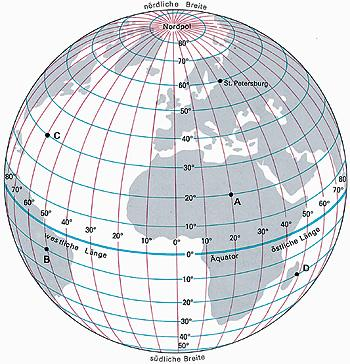
\includegraphics{gradnetz.jpg}
\caption{Das Gradnetz der Erde}\label{gradnetz}
\end{figure}

\noindent Beschrieben wird ein Punkt auf der Erde durch gedachte Kreise um den Globus, welche Senkrecht zueinander stehen. Insgesamt existieren 180 Breitenkreise (Richtung Ost-West) und 360 Längenkreise (Richtung Nord-Süd). Die Abweichung von den beiden Referenzkreisen Äquator und Nullmeridian wird in Grad östlicher/westlicher Länge und nördlicher/südlicher Breite angegeben. Als Äquator ($0^\circ$ nördliche/südliche Breite) wird der Breitenkreis bezeichnet, auf welchem die Erdachse senkrecht steht. Der Nullmeridian ($0^\circ$ westliche/östliche Länge) ist der Längenkreis, welcher durch die britische Stadt Greenwich verläuft.\newline Weitere wichtige Koordinatensysteme sind die Gauß-Krüger und UTM-Koordinaten. Die Vorteile dieser Systeme ist, dass sich eine geografische Position direkt ablesen lässt. Geografische Koordinaten erschweren dies bedingt durch die sich verändernden Abstände zwischen den Längenkreisen in zunehmender Nord- oder Südrichtung.


\section{Qualitätsmerkmale}
Ein wichtiger Forschungszweig ist die automatische Beurteilung von Qualitätsmerkmalen von Geodaten hinsichtlich einer bestimmten Fragestellung.
Ein geeignetes Maß ist die gewichtete Summe verschiedener Datenmerkmale, welche in der aktuellen ISO-Norm \textit{ISO 19157:2013}\footnote{https://www.iso.org/standard/32575.html} spezifiziert sind. Die folgende Auflistung ist eine informelle Beschreibung der oben genannten Norm durch Fragestellungen und Beispiele:


\begin{itemize}
\item \textbf{Vollständigkeit}
\begin{itemize}
\item \textbf{Datenüberschuss} -
Enthält der Datensatz mehr Objekte und Beziehungen als angegeben?
\item \textbf{Datenmangel} - Enthält der Datensatz weniger Objekte und Beziehungen als angegeben?
\end{itemize}
\item \textbf{Logische Konsistenz}
\begin{itemize}
\item \textbf{Konzeptuelle Konsistenz} - 
Wurde die Gestalt des Datenmodells bei Aktualisierungen nicht verändert?
\item \textbf{Wertekonsistenz} - Sind alle Werte sinnvoll?
\item \textbf{Formatkonsistenz} Passen die Daten zu angegebenen physikalischen Einheiten?
\item \textbf{Topologische Konsistenz} 
Bleiben topologische Beziehungen bei Änderungen des Datensatzes bestehen (Der botanische Garten befindet sich im Umkreis von 1km von der HHU)?
\item \textbf{Geometrische Konsistenz} - Ist der digitalisierte Datensatz geometrisch sinnvoll und widerspruchsfrei?
\end{itemize}
\item \textbf{Positionsgenauigkeit}
\begin{itemize}
\item
\textbf{Äußere Genauigkeit} - Wie gut stimmen die Koordinatenwerte des Datensatzes mit den wahren Koordinaten überein?
\item \textbf{Innere Genauigkeit} - Wie gut stimmen die relativen Positionen von Objekten zueinander mit den wahren relativen Positionen überein?
\item \textbf{Rasterdatengenauigkeit} - Wie gut stimmen die Rasterdatenpositionswerte mit den wahren Werten überein?
\end{itemize}
\item \textbf{Zeitliche Genauigkeit}
\begin{itemize}
\item
\textbf{Genauigkeit von Zeitmessungen} - 
Wie genau ist die Zeitangabe (minutengenau, taggenau)?
\item \textbf{Zeitliche Konsistenz} - Ist die Reihenfolge der Ereignisse korrekt?
\item
\textbf{Zeitliche Gültigkeit} - Ist der Datensatz in Bezug auf das geforderte Zeitformat korrekt?
\end{itemize}
\item \textbf{Thematische Genauigkeit}
\begin{itemize}
\item
\textbf{Richtigkeit der Klassifikation} - Stimmen Objekte, oder ihre Attribute mit den zugewiesenen Klassen überein, z. B. Zuordnung zu Fluss, statt zu Weg
\item \textbf{Richtigkeit nichtquantitativer Attribute} - Beispiel: Ist das Grundstück wirklich eine Bananenplantage?
\item \textbf{Genauigkeit quantitativer Attribute} - Beispiel: Ist die Fläche des Grundstücks korrekt?
\end{itemize}
\end{itemize}

Viele der oben genannten Punkte lassen einen subjektiven Spielraum für die Bewertung zu. Sowohl Skalierungen als auch Gewichtungen sind nicht eindeutig definiert, was einen Vergleich verschiedener Datensätze erschwert. Aus diesem Grund ist eine algorithmische Interpretation in Kombination mit verfahren der künstlichen Intelligenz hilfreich. So ließe sich aus der Norm ein universeller und allgemeingültiger Indikator zur Bewertung der Datenqualität ermitteln.


\section{Georeferenzierung}
\subsection{Definition}
Unter dem Vorgang der Georeferenzierung,versteht man die Zuweisung raumbezogener Informationen, auch Georeferenz genannt, zu einem Datensatz.

Es gibt folgende vier Arten der Georeferenzierung:

\begin{itemize}
\item Adresskodierung
\item Geotagging 
\item Kartenkalibrierung 
\item Rektifizierung
\end{itemize}

\subsection{Adresskodierung}
Bei der Adresskodierung wird dem Datensatz eine Postanschrift zugewiesen und somit ein indirekter Raumbezug hergestellt. Mithilfe geokodierter Adressen lassen sich funktionale zusammenhänge zwischen Daten, Postanschrift und Adresse herstellen und somit ressourcenschonende und schnelle Zugriffe ermöglichen.
\subsection{Geotagging}
Als Geotagging bezeichnet man das Einfügen eines Attributes (Geotag) inkl. Realweltkoordinate in einen raumbezogenen Datensatz wie ein Bild oder eine Website. Dies ist bei der räumlichen Einordnung der Information hilfreich.
\subsection{Kartenkalibrierung}
Bei der Kartenkalibrierung wird ein räumlicher Datensatz ohne Realkoordinatenbezug mithilfe einer Transformationsvorschrift im Bezug auf die Realwelt so orientiert, dass sich die Koordinaten des Bildes in Realweltkoordinaten einfach umrechnen lassen.
\subsection{Rektifizierung}
Bei der Rektfizierung werden geometrische Verzerrungen in räumlichen Daten entzerrt, indem jedem Datum eine Realweltkoordinate zugeordnet wird.


\subsection{Bestimmung einer Transformationsvorschrift}

Um eine Transformationsgleichung zu finden, werden in der Regel Passpunkte verwendet. Die Passpunkte müssen im Datensatz eindeutig zu erkennen sein. Die Koordinaten der Passpunkte im Realweltkoordinatensystem sind entweder bekannt oder werden einem Referenzdatensatz entnommen. Bei Vektordaten werden die Koordinaten abgegriffen oder interpoliert. Bei Bilddaten werden die Bildkoordinaten der Passpunkte gemessen. Die Transformation sollte unter Berücksichtigung der Abbildungsgeometrie bestimmt werden. Bei Fotos ist somit die Zentralprojektion zu berücksichtigen, bei Karten der entsprechende Kartennetzentwurf. Das automatische Finden von Gemeinsamkeiten in digitalen Bildern und die Bestimmung der Transformation wird in der Bildverarbeitung Bildregistrierung genannt. Die Registrierung von Laserscanning-Punktwolken kann mit dem ICP-Algorithmus erfolgen.\footnote{https://de.wikipedia.org/wiki/Georeferenzierung}

Mark Erweiterungen, implementierungen sinnvoll?

\section{Geoinformationssysteme}
Ein Geoinformationssystem ist eine Software, mit welcher Geodaten erfasst, verwaltet, analysiert und ausgegeben werden können.

Man unterscheidet bei der Abfrage von Daten unter folgenden verschiedenen Typen:
\begin{itemize}
\item Alphanumerische Daten (Attribute als Text oder Zahlen)
\item Text-Dokumente 
\item Multimediale Informationen, wie Videos, Audiosequenzen, Animationen 
\item Fotos, Scans, Satellitenbilder
\end{itemize}

Der Unterschied zu einer Datenbank ist, dass jedes Sachdatum einen expliziten Raumbezug hat, über welchen die Selektion erfolgt. In einer Datenbank erfolgen Zugriffe stattdessen über Schlüsselattribute. Eine weitere Stärke eines GIS ist die grafische Aufbereitung der Daten zur anschaulich-interaktiven Analyse.

Beispiele für solche räumlichen Analysewerkzeuge sind Routenfindung, räumliche Suche. Ein implementiertes Kartografiesystem ermöglicht zudem das markieren von Punkten und Linien, färben von Flächen und die Anzeige und Überlagerung verschiedener Ebenen.

\subsection{Geoobjekte}
Ein Geoobjekt ist ein tatsächlich auf der Erde vorhandenes Objekt, welches durch Geodaten eindeutig referenziert wurde. Man unterscheidet zwischen Gegenständen und Sachverhalten. Gegenstände sind konkrete, visuell wahrnehmbare Erscheinungen auf der Erdoberfläche. Sachverhalte dagegen sind nicht sofort visuell wahrnehmbar, sondern bezeichnen Beziehungen zwischen Gegenständen oder die Interaktion mit der Umwelt und Oberflächengestalt.
Außerdem unterscheidet man zwischen verschiedenen Arten der Datenspeicherung:
\begin{itemize}
\item Flächenhafte Daten
\item Linienhafte Daten
\item Punkthafte Daten
\end{itemize}
Je nach Kartenmaßstab, Auflösungstyp und Speichertyp (digital/analog) werden Daten unterschiedlich repräsentiert. So wird beispielsweise ein flächenhafter quadratischer Gebäudekomplex (10*10 Meter) auf einem Satellitenfoto mit dem Maßstab 1:10.000 nur noch als Punkt wahrgenommen. Linienhafte Daten bieten sich vor allem bei Flüssen, Straßen, Wasser-Land-Grenzen, starken Flankensteigungen usw. an.

\subsection{Modellierung von Geoobjekten}
Die vier informationstechnischen Dimensionen zur Modellierung von geografischen Informationssystemen sind:
\begin{itemize}
\item Geometrie (Ort des Objekts)
\item Topologie (Lage der Objekte relativ zueinander)
\item Semantik (Bedeutung des Objekts im fachspezifischen Kontext, z.B. gut-schlecht, viel-wenig, groß-klein)
\item Dynamik (Änderung des Objekts im zeitlichen Verlauf)
\end{itemize}
Jedes unikate Objekt gehört zu einer Objektklasse, in welcher es nach den oben genannten vier Kriterien beschrieben und mit anderen Objekten der Klasse verglichen wird. Jedes der Objekte besitzt einen eindeutigen Schlüssel zur Identifikation. Möglichkeiten zur Klassifizierung und Clustering von Geoobjekten werden in den folgenden Kapiteln vorgestellt.\newline
Der Ort eines Geoobjektes kann auf zwei verschiedene Arten beschrieben werden:
\subsection{Rastermodell}
Eine analoge topografische Karte oder Zeichnung digitalisiert und in quadratische Gitterzellen aufgeteilt, welche alle über die gleiche Semantik verfügen. Diese Semantik wird stellvertretend durch eine Matrix beschrieben, welche für jede Gitterzelle eine numerische Pixelwertinformation enthält.\footnote{https://de.wikipedia.org/wiki/Geoobjekt}
\begin{figure}[H]
\centering
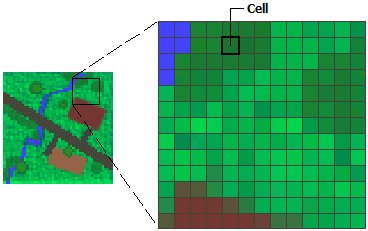
\includegraphics{raster.png}
\caption{Rastermodell-Zoom \protect\footnotemark}
\end{figure}
\footnotetext{http://desktop.arcgis.com/de/arcmap/10.3/manage-data/raster-and-images/what-is-raster-data.htm}
\noindent
Diese Pixelinformationen repräsentieren Daten wie  Temperatur, Höhe, Vegetationsdichte, Landnutzung, Bodenbeschaffenheit. Rasterdaten werden in der Regel als Bilddatei gespeichert (BMP, GIF, JPEG).
\newline
Die Rastergeometrie eignet sich gut zur Beschreibung flächiger, homogener Sachverhalte. Die einfache Struktur bietet viele Vorteile, aber auch Nachteile: \newline
\textbf{Vorteile}
\begin{itemize}
\item Einfache Datenstruktur 
\item Geeignet für räumliche und statistische Analyse
\item Alles ist einheitlich speicherbar (Punkte, Linien, Polygone)
\item Überlagerung von Ebenen sehr schnell und einfach
\end{itemize}
\textbf{Nachteile}
\begin{itemize}
\item Genauigkeitsverlust beim Scannen und Neustrukturieren
\item Endliche Auflösung => räumliche Ungenauigkeit
\item Pixelwerte haben keine Beziehung zueinander
\item Hoher Speicheraufwand bei Hoher Auflösung, keine Kompression möglich.
\end{itemize}

\subsection{Vektormodell}
Im Gegensatz zu Rasterdaten werden Vektordaten bei linien- und punkthaften Informationen eingesetzt, also Informationen, die sich nicht mit homogener Eigenschaft über die gesamte Karte verteilen. Man nennt solche Informationen auch Features. Beispiele hierfür sind Straßen, Staatsgrenzen, Gewässergrenzen, Höhenlinien, Flüsse, Bäume.
\newline
Eine Punkthafte Vektorinformation wird auch als Vertex bezeichnet. Dieser beschreibt eine Raumlage durch Angabe einer (x,y,z)-Koordinate und ein dazugehöriges Attribut, welches die Art des Punktes beschreibt, z.B. Baum oder Laterne:

\begin{figure}[H]
\centering
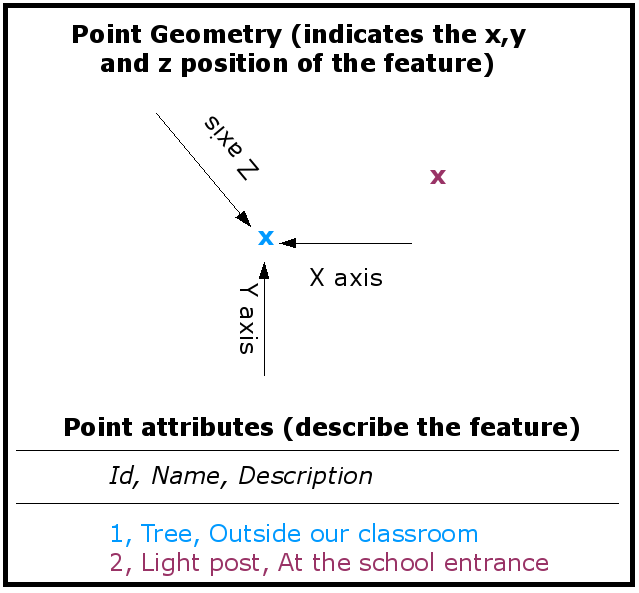
\includegraphics[scale=0.6]{vertex.png}
\caption{Punkt-Feature \protect\footnotemark}
\end{figure}

\footnotetext{https://docs.qgis.org/2.8/de/docs/gentle\_gis\_introduction/vector\_data.html}

\noindent
Punkteverläufe wie Straßen werden durch sogenannte Polylinien beschrieben. Diese bestehen aus mehreren miteinander verbundenen Vertices. Im Kreis laufende Polylinien bezeichnet man auch als Polygone:

\begin{figure}[H]
\centering
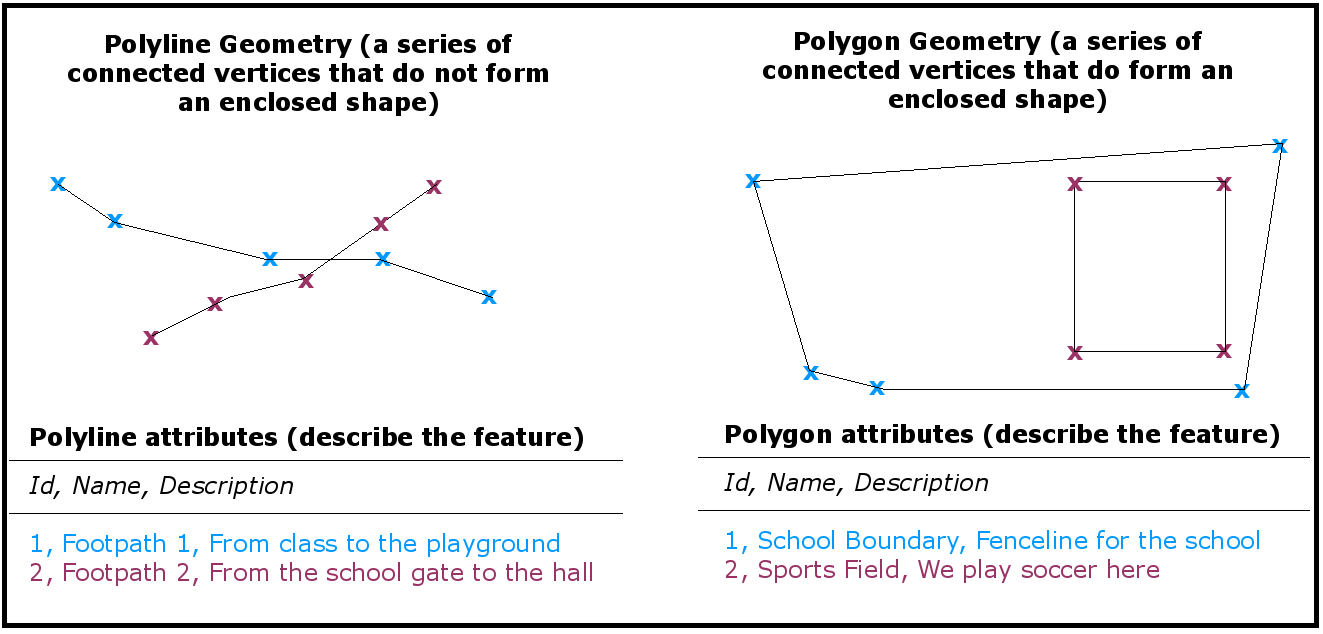
\includegraphics[scale=0.6]{poly.png}
\caption{Polylinien und Polygone \protect\footnotemark}
\end{figure}

\footnotetext{https://docs.qgis.org/2.8/de/docs/gentle\_gis\_introduction/vector\_data.html}

\noindent
Wie auch bei Rasterdaten gibt es bei Vektordaten nicht nur Vorteile, sondern auch Nachteile.\footnote{http://romanharcke.de/geoinformationssysteme-geodaten-kapitel-4/}\newline
\textbf{Vorteile:}
\begin{itemize}
\item Unendliche Linienauflösung und sehr hohe Genauigkeit
\item Beschreibung von mehreren einzigartigen Features in nur einer Ebene möglich
\item Geringer Speicherbedarf
\item Einfache Erzeugung von Topologie (Knoten, Kanten, Flächen)
\item Gute Performance
\item Ermöglicht Attributierung und Objektdefinitionen
\end{itemize}
\textbf{Nachteile:}
\begin{itemize}
\item Flächenhafte Informationen können nicht gespeichert werden 
\item Durch Scannen können diese Daten nicht erzeugt werden. Es bedarf hier einer Raster-Vektorwandlung (Hoher Erfassungsaufwand)
\item Hoher Rechenaufwand bei Verschneidungen
\end{itemize}

\section{Beispiele von Raster und Vektordaten}
Geodaten müssen heutzutage nicht mehr selbständig erstellt werden. Es gibt eine Vielzahl an staatlichen und privaten Institutionen, welche Ihre Daten kostenlos bereitstellen. So lassen sich zahlreiche Inhalte im ESRI Shapefile Vektordateiformat finden, welches als Quasi-Standard für Desktop-GIS gilt.\footnote{https://de.wikipedia.org/wiki/Shapefile}
\noindent
Der Datensatz \textit{Natural Earth}\footnote{http://www.naturalearthdata.com/} ist eine Abbildung der Erde im Maßstab 1:10 Millionen. Er ist sowohl als SHP-Vektordatei als auch als Tiff-Rasterbild verfügbar.

\noindent Ein ESRI Shapefile besteht aus mindestens drei Dateien zur Speicherung der Geometriedaten, Sachdaten und der Geometrieindizierung zur Verknüpfung von Geometrie und Sachdaten (.shp, .dbf, .shx). Die Geometrie eines Shapefile definiert sich aus nur 4 verschiedenen Formdatenstrukturen: Punkte, Linien, Flächen (Polygone) und Multipunkte.\footcite{http://www.esri.com/library/whitepapers/pdfs/shapefile.pdf}

\begin{figure}[H]
\centering
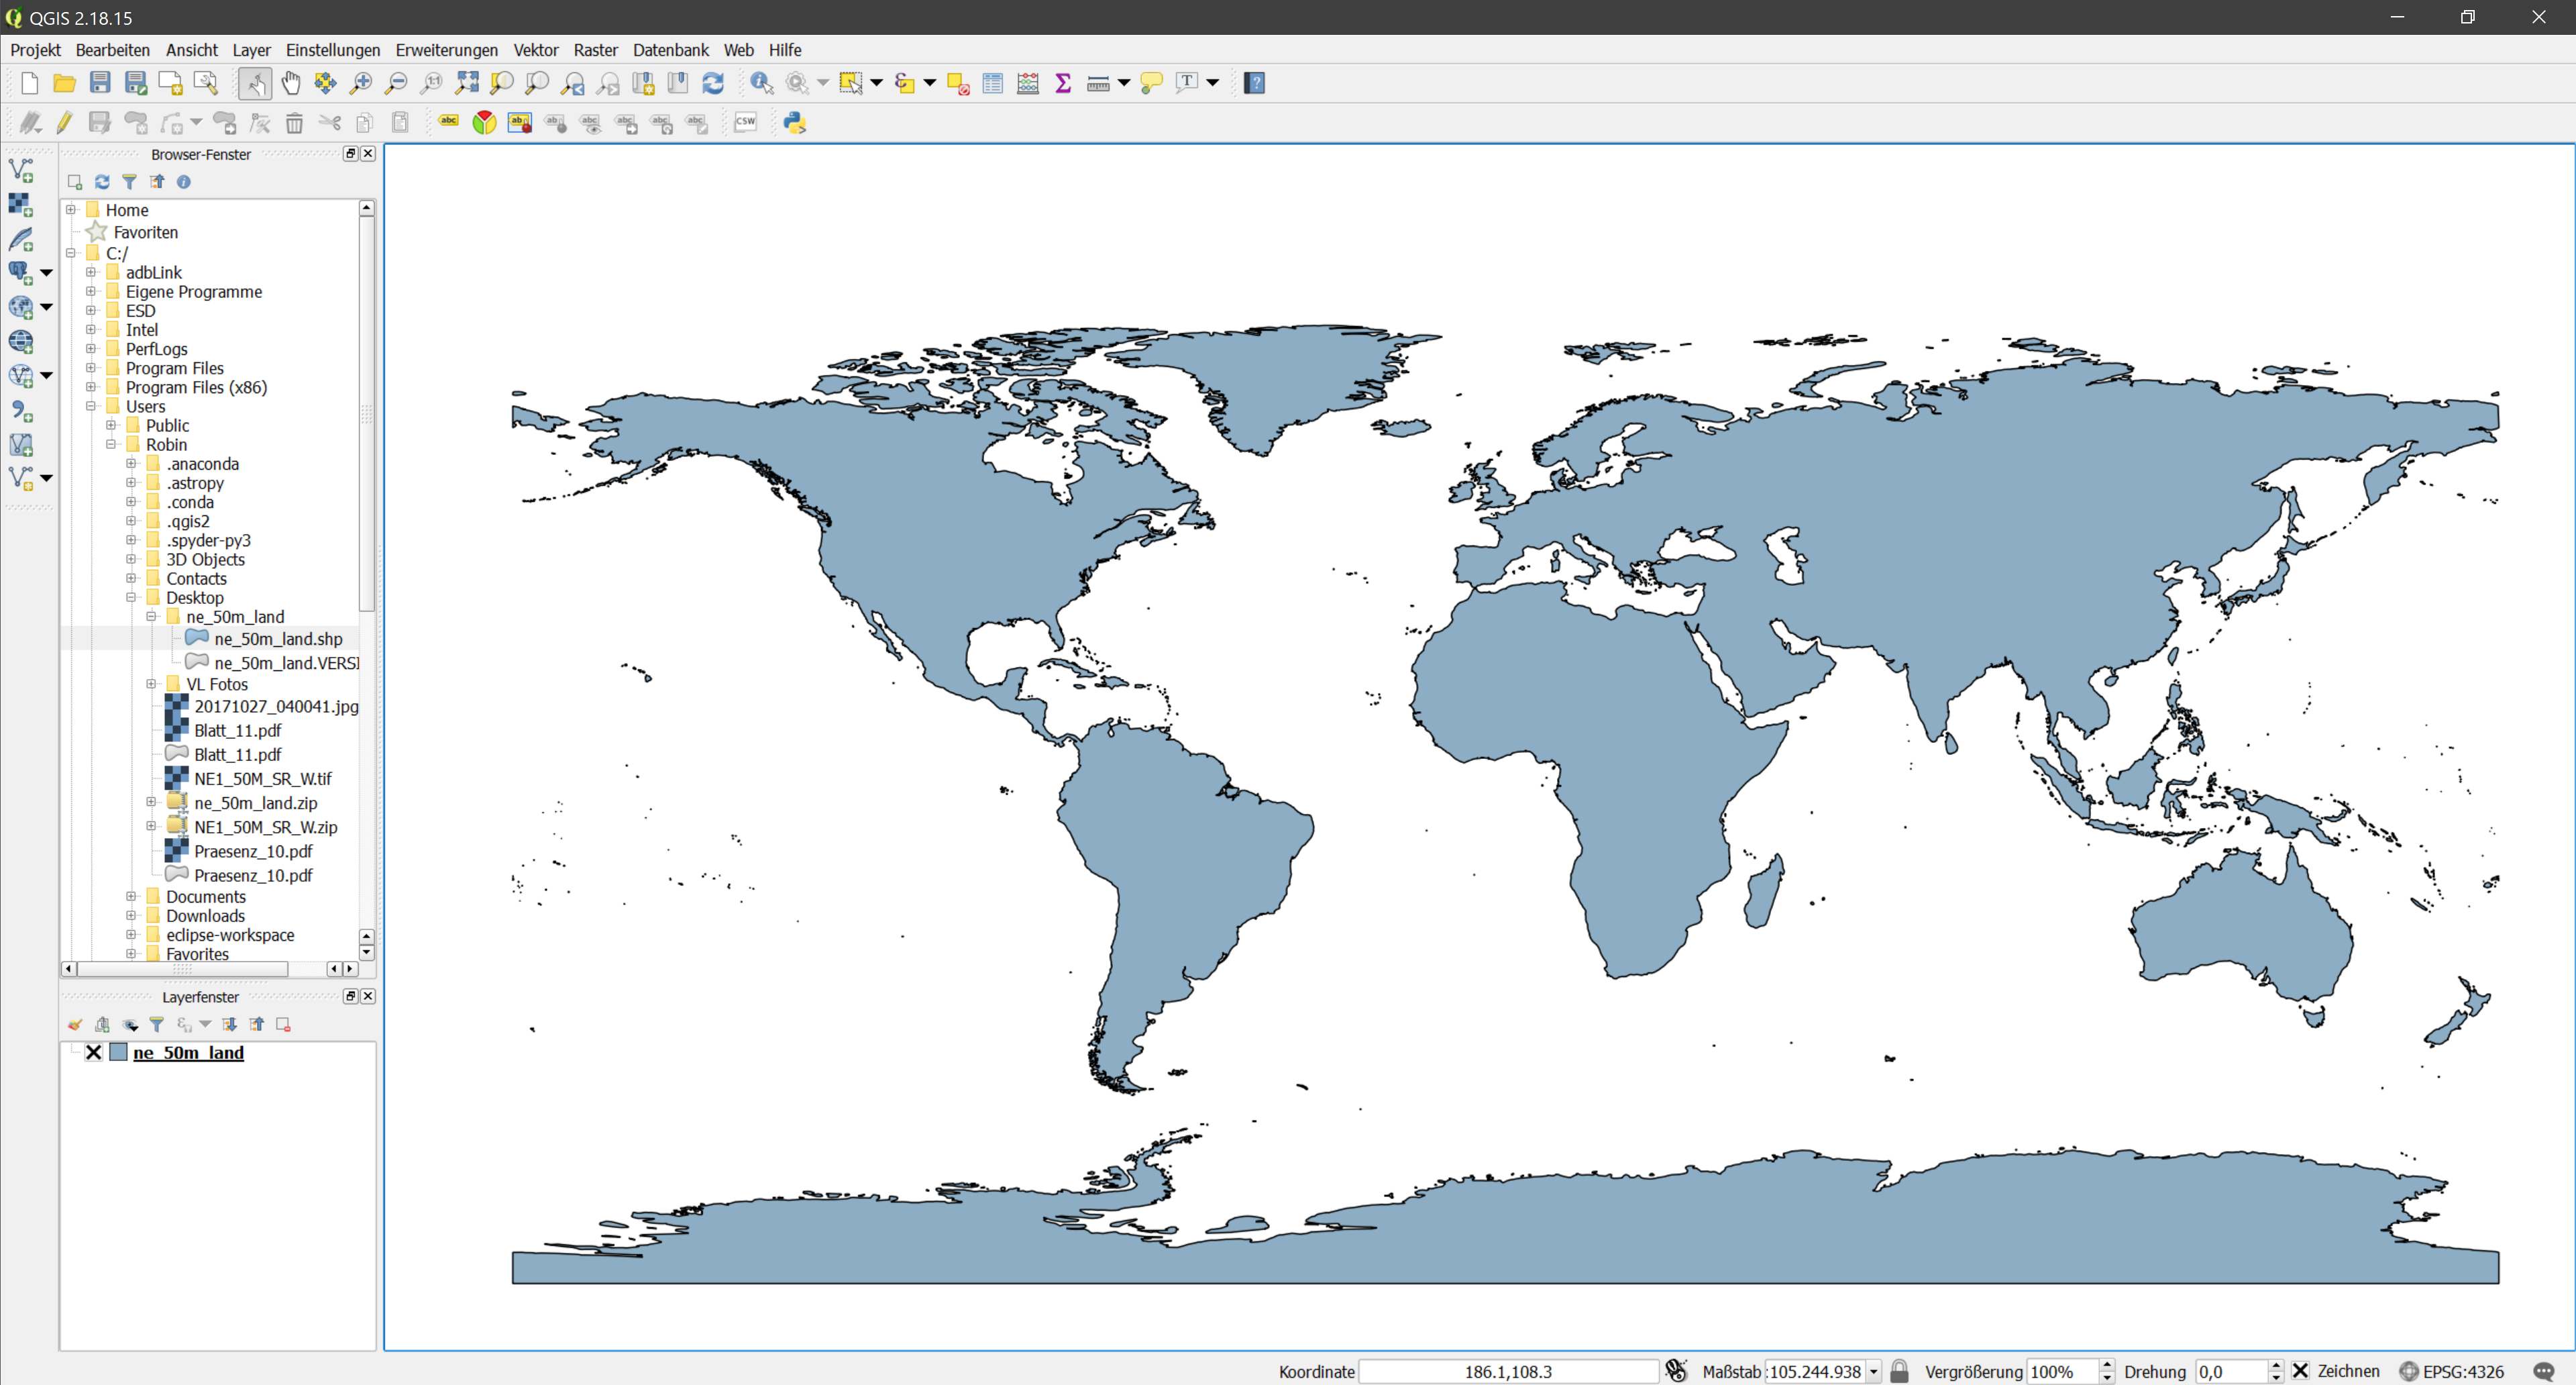
\includegraphics[scale=0.23]{gis.png}
\caption{.shp-Geometriedatei in dem Geoinformationssystem QGIS dargestellt \protect\footnotemark}
\end{figure}
\footnotetext{https://www.qgis.org/de/site/}
\noindent
Leider eignen sich Vektordaten nicht zur Klassifikation von Features mit Hilfe von Deep Learning wie z.B. Convolutional Neural Networks (CNN), sondern stellen viel mehr das Ergebnis einer Rasterbildanalyse dar. Aus diesem Grund beziehen sich folgende Kapitel im Kontext von Geodaten immer auf Rasterdaten und Bildausschnitte.
\newline
Das dem Datensatz zugehörige farbige Rasterbild inklusive Schummerung (räumliche Schattierung), Wasser und Flüssen sieht so aus:

\begin{figure}[H]
\centering
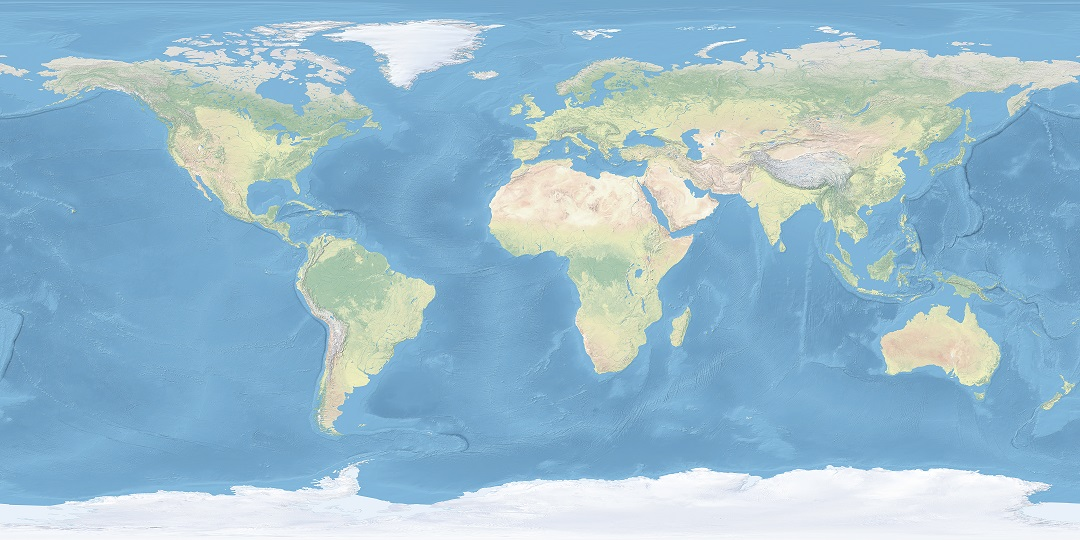
\includegraphics[scale=0.4]{raster_nat_earth.png}
\caption{Rasterbild des Natural-Earth-Datensatzes \protect\footnotemark}
\end{figure}
\footnotetext{http://www.naturalearthdata.com/downloads/10m-raster-data/10m-natural-earth-1/}




\section{Algorithmen in der Geoinformatik}

\section{Verschiedene Arten und ihre Anwendungszwecke}


\chapter{Geoanalyse}
\section{Beispiele}
\section{Offene Probleme}

\chapter{Neuronale Netzwerke}
\section{Anwendungszwecke}
\subsection{Vorhersage von Städtewachstum}
\section{Tensorflow}
\section{Anwendung auf Satellitendaten}


\chapter{Clusteringverfahren}
\section{Probabilistisches und Possibilistisches Clustering}
\subsection{FCM und PFCM}
\subsection{Vorraussetzungen für die Anwendung auf Geodaten}
\subsection{Eigener Algoritmus (noch ohne Name)}
\section{CVI}
\subsection{NPC}
\subsection{FHV}
\subsection{Otsu-Binarisierung}
\subsection{VAT-Algorithmus}
\section{Clustering auf unvollständigen Daten}
\chapter{Forschungsbedarf}
\section{Ausblick - Mein Thema für die Masterarbeit}

\vfill
\end{document}